\section{Introduction}
\label{sec:intro}
\subsection{DNA Replication, Damage and Repair -  An Overview}
All cells experience a large number of DNA modification events per day that have to be processed and repaired in order for the cell to replicate its genome with as few errors as possible to guarantee proper function of daughter cells. Though mutations are not favoured on a large scale, lower levels of mutations in the genome of differentiated cells can have useful effects on daughter cells such as gains of protein functions to adapt better to the environment. Additionally, cell specialization relies in its core on retaining preferable mutations in a cell population or a tissue.\\
Many of those modifications occur spontaneously but some DNA lesions are caused by endogenous or environmental factors such as reactive oxygen species (ROS), ultraviolet light (UV), ionizing radiation (IR) as well as chemical agents and drugs \citep{Loeb.2008}. ROS in particular are introduced to the cell by metabolic processes such as respiration (via Hem proteins, Cytochrome P \textsubscript{450} and the reaction with metal ions) or from exogenous sources such as smoking and the uptake of ROS with nutrients.\\
\begin{figure}[H]
        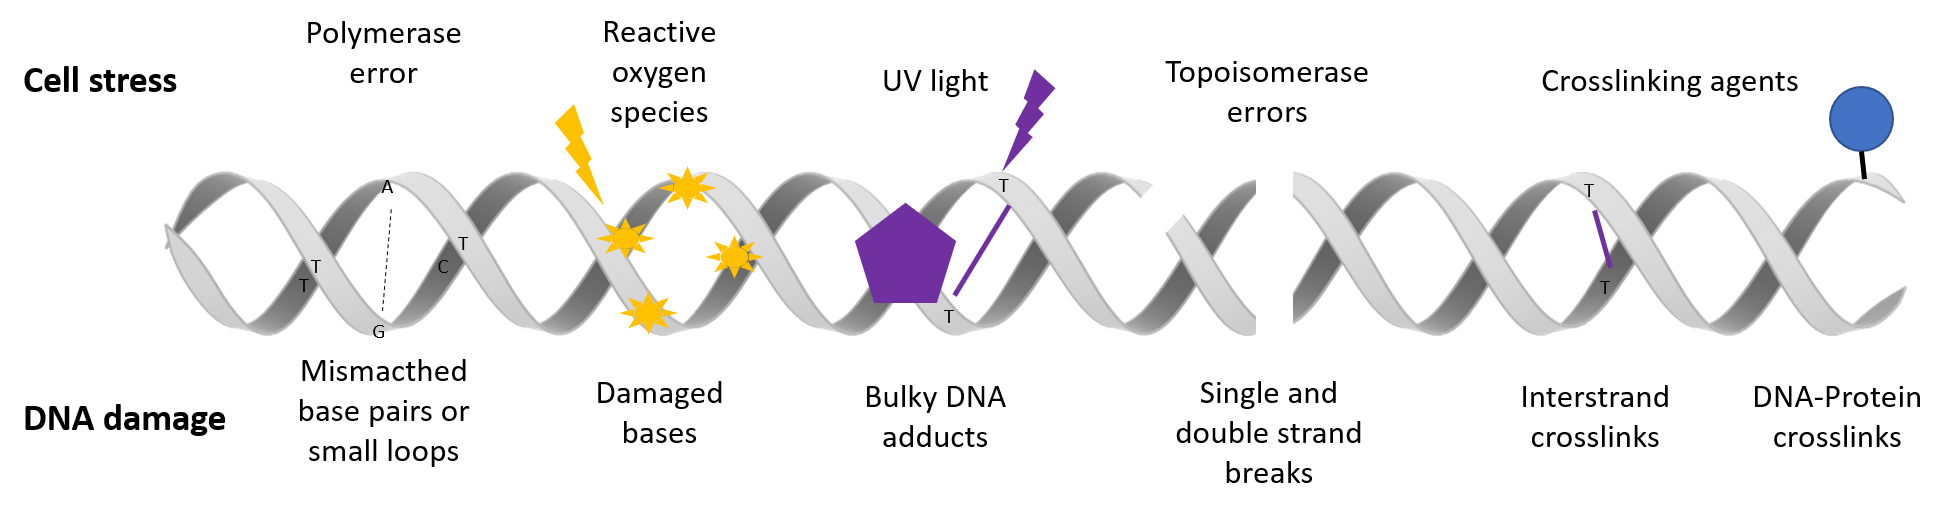
\includegraphics[width=\textwidth]{resources/images/Intro/damageTypes.png}
        \caption[Overview of DNA damage effectors and their main lesions]{\textbf{Overview of DNA damage effectors and their main lesion.} Errors caused by DNA polymerases are limited to misincorporated bases or small insertions or deletions whereas reactive oxygen species cause damaged bases or single strand breaks. UV light often leads to DNA adducts of larger sizes. Crosslinking agents such as Psoralen can introduce links between the DNA strands (Interstrand Crosslink) or between a DNA strand and a bound Protein (DNA-Protein Crosslinks). Modified from \cite{Massey.2018}.}
        \label{fig:damOverview}
\end{figure}
Some chemical DNA damage inducers such as mitomycin C or malphalan are used as cancer therapeutics due to their alkylating properties. Additionally, crosslinking agents such as psoralen, introduce covalent crosslinks between DNA strands (interstrand crosslinks, ICL) \citep{Ciccia.2010} wherease other crosslinkers such as formaldehyde can form DNA-Protein-Crosslinks (DPC). Formaldehyde can be a byproduct of DNA methylation and therefore, DPCs are relatively common DNA lesions. Inhibition of topoisomerases can also cause enzymatically derived DPCs by covalently linking the topoisomerases to the DNA \citep{KlagesMundt.2017}.\\
The inability to repair those alterations leads to pathological phenotypes such as senescence, cancer and cell death. Additionally, accumulation of damaged DNA destabilizes genomic integrity. To prevent an accumulation of lesions they are individually detected and repaired via a specific pathway using a multitude of proteins with varying degrees of specificity. Though many proteins are involved in the repair of different lesion types, each lesion type itself shows a specific footprint over the course of its detection and repair. Some DNA damages are detected during replication and immediately repaired where as others are detected via replication independent factors that induce on-the-fly repair mechanisms. 
\\
\\
As mentioned, changes in the blueprint of life are a key feature of evolution that facilitate diversity but it is crucial to keep those changes at equilibrium with the perpetuation of genetic information. In a multicellular organisms it is possible to transmit genomic instability introduced by mutations to a new generation of cells (gametic cells) and structural components of the organism (somatic cells). It has been shown in humans that genomic instability in somatic cells is closely related to cancer, and to avoid that cells may die. This controlled cell death however has been associated with the trigger of processes that are related to organism aging. The importance of DNA repair mechanisms can be demonstrated in a number of human syndromes that are characterized as being caused by defective DNA repair processes. One of those syndromes is xeroderma pigmentosum (XP) which is described as a defect in nucleotide excision repair (see \ref{sec:polblock}; NER). NER normally removes lesions that are caused by UV exposure which in XP patients leads to a high frequency of tumors in exposed areas of the skin as well as - in more severe cases - developmental problems, neurodegeneration and premature aging. The more severe symptoms are also associated with Cockayne syndrome that is also characterized as a defect in NER \citep{Menck.2014}.  Ataxia telangiectasia or Louis-Bar-Syndrom shows similar symptoms with the addition of motor impairments and an immunological imbalance but is characterized by a mutation in the \textit{ATM}-gene which codes for a protein kinase that is involved in double strand break (DSB) repair. ATM is expressed ubiquitously but seems to be especially involved in the maintenance of Purkinje cells in the cerebellum and other structures of the human brain.  Other human syndromes are caused by more complex mutation patterns, one of them being Fanconi anemia (FA). FA is caused by mutations in at least one of 15 genes involved in the repair of interstrand crosslinks (ICL) that lead to developmental imbalances such as malformed appendages as well as skin discolorations and - in serious cases - bone marrow failure.\\\\
\begin{wrapfigure}{l}{0.6\textwidth}
    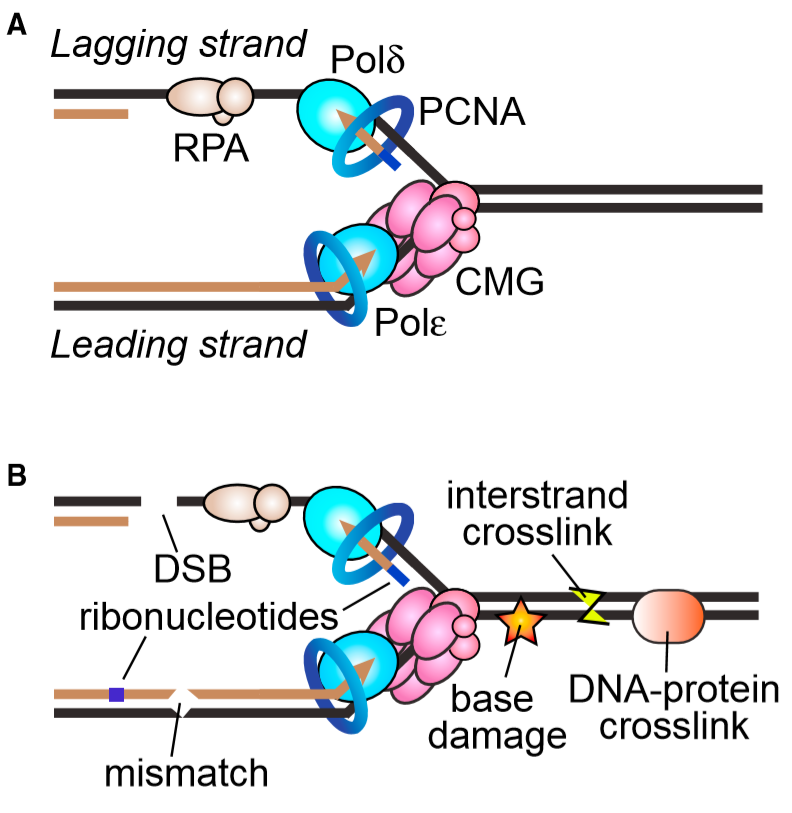
\includegraphics[width=0.56\textwidth]{resources/images/Intro/replicationfork.png}
    \caption[Resolution of DNA Lesions via Replication-Coupled Pathways]{\textbf{Resolution of DNA Lesions via Replication-Coupled Pathways.}\\A) Simplified schematic of a eukaryotic replication fork.\\B) Lesions generated or encountered by the replisome.\\\citep{Cortez.2019}}
    \label{fig:replicationfork}
\end{wrapfigure}
All of the syndromes briefly introduced above share an elevated risk for cancer though based on the inability to repair one or more types of DNA lesions which leads to genomic instability and/or uncontrolled growth of affected cells. Understanding the mechanisms of the repair of DNA lesions as well as the pathways regulating them is crucial for preventing cancer and treating syndromes such as the ones mentioned above. Though numerous studies have been published over the last decades that investigated and resolved the mechanisms behind the repair of individual DNA lesions there is no comprehensive resource available to researchers that focuses on DNA repair on a systemic level. Many proteins involved in the repair of DSBs are also associated with the repair of ICLs, even though lesion detection as well as regulation and recruitment of lesion specific proteins differs greatly between those mechanisms. Due to this we wanted to look at the interactions between each repair mechanism to resolve DNA repair as a system instead of a collection of individual pathways. To do so we applied graph theory to a collection of chromatin proteomic data investigating the recruitment of proteins involved in DNA repair and replication in \textit{Xenopus} egg extracts (see \ref{sec:extracts}) to specifically damaged DNA templates. Each of the sets used in this thesis has been - be it already published or still in progress - used to resolve or improve the understanding of a single repair mechanism but has never been comprehensively compared to experiments investigating other repair mechanisms. As will be explained in more detail in section \ref{sec:extracts} the \textit{Xenopus} egg extract systems have in the past only been used to investigate mechanisms that are dependent on replication of the DNA template used. Due to this most of this thesis will focus on replication coupled DNA repair mechanisms (see Figure \ref{fig:replicationfork}).

\subsection{DNA Replication and the Cell Cycle}
To understand how DNA lesions are repaired in a replication dependent manner, one has to understand DNA replication itself. Eukaryotic cells undergo different stages during their life cycle to ensure an efficient and error-free cell division that leads to the formation of two identical and functioning daughter cells. A key mechanism during this cycle is the replication of the genome and therefore the error-free synthesis of new DNA molecules based on a template. Before we go into detail about how replication is initiated and carried out, we want to give a short introduction to the cell cycle of eukaryotic cells and the differences between model organisms and humans.

\subsubsection{The Cell Cycle: A brief Overview}
The circular process of cell life and division is differently regulated for each type of differentiated cell, where some continue to divide indefinitely and others differentiate to the point of being fixed in one phase until cell death is induced. Figure \ref{fig:cellCycle} shows a schematic of the stages of the cell cycle. It consists of two mayor phases - M-Phase and Interphase - where the latter can be split into three main stages that make up the bulk of the cells life (see figure \ref{fig:cellCycle}). 
\begin{figure}
    \centering
    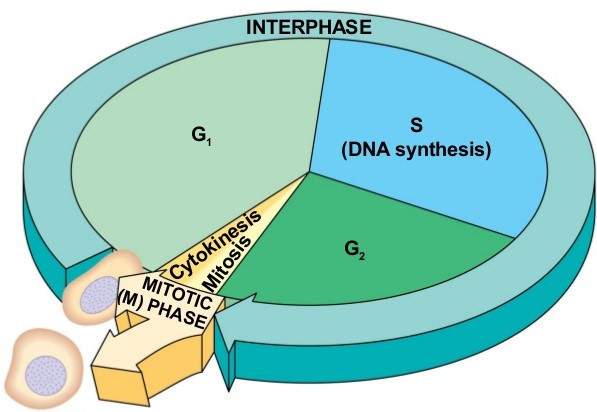
\includegraphics[width=.68\textwidth]{resources/images/Intro/cellCycle.jpg}
    \caption[Schematic view of the cell cycle]{\textbf{Schematic view of the cell cycle. }Cells experience 5 distinct phases during their life cycle. In G\textsubscript{1} the cell prepares to replicate its DNA in S-Phase and remains in G\textsubscript{2} until it has to divide its nucleus during mitosis. The cell cycle is completed after one maternal cell divides into two daughter cells during cytokinesis.\\\citep{Campbell.2015}}
    \label{fig:cellCycle}
\end{figure}
Simplified, Interphase starts with a stage called G\textsubscript{1} where all DNA is organised in a condensed form called heterochromatin that has to be unpacked to be replicated during the following S-stage. During S-phase DNA is replicated and the replicated molecules are attached to each other on their centromers to form so called sister-chromatids that are stored in the nucleus during the following G\textsubscript{2} phase. Differentiated cells that are not supposed to undergo mitosis anymore then enter G\textsubscript{0} until signalled otherwise or until cell death (not pictured in Figure \ref{fig:cellCycle}). 
Cells that are supposed to continue in cell division enter M-Phase which consists of Mitosis and Cytokinesis. During Mitosis, the nucleus of a cell is dissolved, the sister-chromatids are separated and transported to different poles of the cell. From there, two new daughter nuclei form to complete Mitosis. 
\begin{wrapfigure}{l}{0.4\textwidth}
    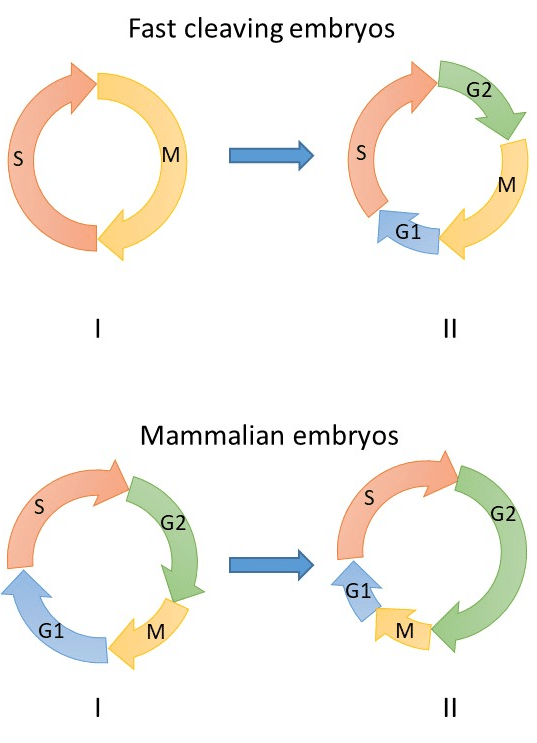
\includegraphics[width=.38\textwidth]{resources/images/Intro/cycleXenHum.png}
    \caption[Different course of fast cleaving VS. mammalian embryonic cell cycles]{\textbf{Different course of fast cleaving VS. mammalian embryonic cell cycles.}\citep{Kermi.2019}}
    \label{fig:XenHumCyc}
\end{wrapfigure}
Cytokinesis completes the cycle by dividing the cytoplasm of the mother cell into two newly generated daughter cells that enter Interphase. These Mechanisms are of course heavily regulated with molecular checkpoints that have to be cleared before entering a new phase. Additionally, regulatory proteins are deployed during S phase that inhibit DNA replication to prevent the cell from replicating its genome more than once. Such regulatory proteins can be used to induce stress in a cell or another system used to study replication and DNA repair (see section \ref{sec:extracts}).\\
Embryonic cell cycles show differences in the presence of phases and proteins in comparison to the cell cycle in adults as well as differences between classes of eukaryotes. Fast cleaving embryos such as \textit{Xenopus laevis} don't undergo G\textsubscript{1} and G\textsubscript{2} during Interphase in their early stages but show relatively short G-Phases and a longer M-Phase than mammalian embryos that start with all four phases and only change the duration of each phase during embryonic development (see Figure \ref{fig:XenHumCyc}).\\
All data used in this thesis was acquired using \textit{Xenopus} cell free egg extracts that can be used to study replication dependent mechanisms of DNA repair. Different extract types are used to study different mechanisms but the details of said extracts will be discussed later.

\subsubsection{Initiation of DNA Replication}
\label{sec:cellcycle}
The replication of DNA based on the template genome of a cell during S-Phase starts with the recruitment of the Origin Recognition Complex (ORC) consisting of six subunits to an Origin of Replication. Per DNA molecule, many origins are loaded with ORC but not all of them are activated. The mechanisms of choosing which origin stays dormant and which will get activated as well as the function of dormant origins is extremely complex and beyond the scope of this thesis. It has been shown that the dormant origins are involved in the maintenance of genomic stability \citep{Alver.2014}.
\begin{figure}[H]
    \centering
    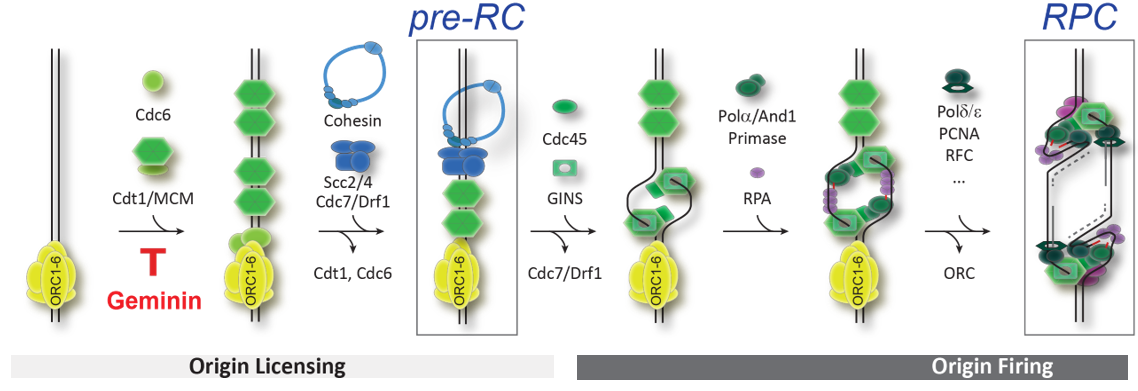
\includegraphics[width=\textwidth]{resources/images/Intro/repIni.png}
    \caption[Mechanisms of Replication Initiation]{\textbf{Mechanisms of Replication Initiation. } The origin recognition complex (ORC) binds to an origin of replication and recruits Cdc6 and the MCM-helicase that is associated with Cdt1. Cdt1 and Cdc6 dissociate from the origin to give way for the recruitment of the Scc2/4 Cdc7/Drf1 tetramer and Cohesins to complete the pre-Replication Complex (pre-RC). The Cdc7/Drf1 dimer is released and Cdc45 in conjunction with the GINS complex is recruited. With this, the origin  is prepared for DNA replication to be initiated. RPA, Primase and Pol\textalpha are then recruited and after release of the ORC other polymerases as well as PCNA are recruited to form the replication complex (RPC) and start replication.\\\citep{Raschle.2015}}
    \label{fig:replication_overview}
\end{figure}
Activated origins are then loaded with Cdc6 as well as the Cdt1/MCM complex. After dissociation of Cdt1 and Cdc6 the MCM helicase complex promotes recruitment of Cohesins and the Cohesin-recruiter proteins Cdc7 and Drf1 to form the pre-Replication Complex (pre-RC). The Cdc7/Drf1 dimer is replaced by Cdc45 and the GINS complex that bind to and activate the MCM helicase to open up the replication fork. DNA polymerases and the primimg protein Primase as well as the ssDNA stabilizing protein RPA are recruited to the now opened replication fork. To finalize the initiation of DNA replication PCNA is loaded and ORC dissociates from the origin. From there on each DNA molecule is replicated with an extremely low error rate until a potential DNA lesion is reached. each type of DNA lesion is detected by different factors and repair using specific molecular mechanisms that will be explained in the section below.\newpage

\subsection{An Introduction to the DNA Damage Response (DDR)}
Quick and accurate replication of DNA in each cell during every cell cycle is crucial for the survival of the cell. Even though the replisome is a very accurate machinery, it does not function error-free.\\\\
DNA replication is enabled by the use of three main polymerases: Pol\textalpha, which incorporates priming nucleotides, Pol\textdelta, which polymerizes the leading strand, and Pol\textepsilon, which polymerizes the lagging strand. These three polymerases are listed in order of descending error-proneness where Pol\textepsilon shows the highest fidelity with only 1 false base incorporations out of 10\textsuperscript{6} bases. 

\subsubsection{Resolution of Polymerase Blockages}
\label{sec:polblock}
Base lesions such as abasic sites, base oxidation and base methylation often pause polymerases in their path. Spontaneous base loss and glycosylase removal of uracil cause about 10,000 - 20,000 abasic sites each day in each human cell whereas all other base lesions form about 20,000 times each day on average. Environmental factors such as UV light can increase the rate of such base lesions dramatically and even though most of them are repaired by replication independent mechanisms such as Base Excision Repair (BER) or Nucleotide Excision Repair (NER), these systems can not always repair them prior to replication fork arrival.\\
The response to a base lesion heavily depends on the template strand the lesion is found in. A lagging strand lesion may stall Pol\textalpha-primase or Pol\textdelta but can not stall the replication fork in total because new primers on the lagging strand lead to a natural skippage of the lesion. The gaps created during those skipping maneuvers are repaired after replication by translesion-bypass polymerases. This lesion-skipping model has not yet been verified in vertebrates because of the difficulty of introducing lagging-strand directed lesions \citep{Goodman.2013}. Lesions on the leading strand however are block Pol\textalpha~more effectively because of the lack of new primers on the strand which leads to a functional uncoupling of the CMG helicase and the DNA synthesis. This uncoupling by itself may not be as problematic as one might expect. It has been shown in \textit{E. coli} that there is little coordination between leading and lagging strand synthesis with or without DNA damage. Additionally, helicase activity is reduced by ~80\% when DNA synthesis stops. This effectively forms a "dead man's switch" that prevents the helicase from unwinding too much DNA ahead of synthesis \citep{Goodman.2013,Marians.2018}. In case of the helicase running too far ahead, repriming of the leading strand occurs within several minutes and does not require a specific primase in \textit{E. coli} which allows replication to resume. The bacterial replisome is capable of skipping leading strand lesions relatively easily whereas the eukaryotic replisome has the ability to skip them to some extend but it seems to prefer usage of a specialized primase called \textit{PrimPol} \citep{Rechkoblit.2016}. An overview of the responses to leading- and lagging strand base damages can be seen in Fig. \ref{fig:lesionskipping}.
\begin{wrapfigure}{r}{0.6\textwidth}
    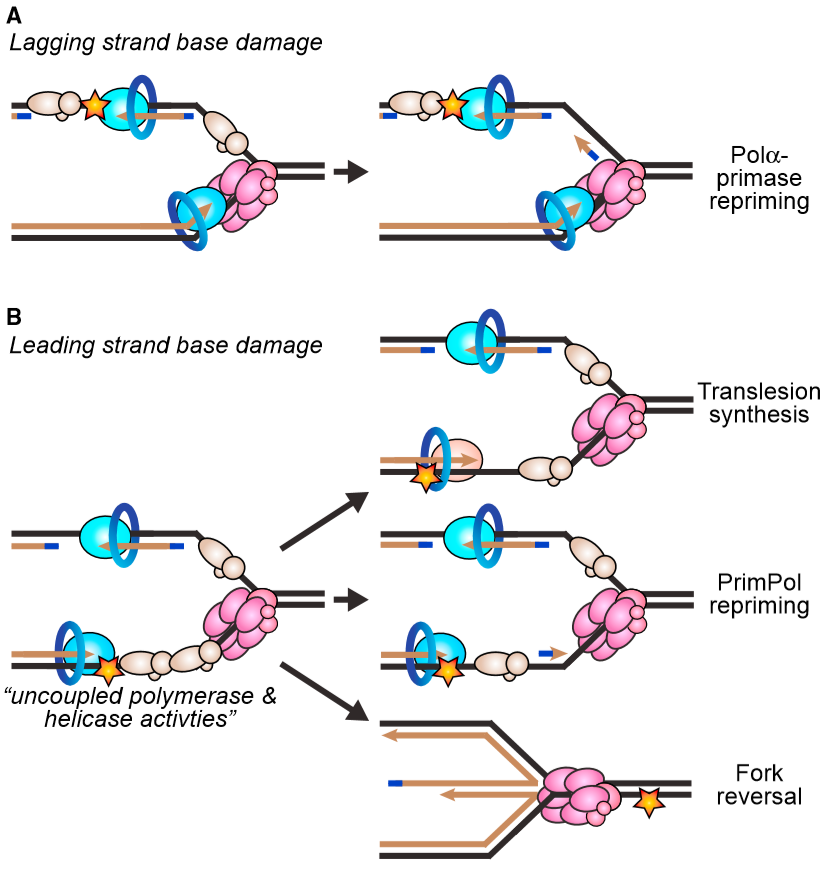
\includegraphics[width=0.58\textwidth]{resources/images/Intro/lesionskipping.png}
    \caption[Schematic of the Response to Leading- and Lagging Strand Base Damage]{\textbf{Schematic of the Response to Leading- and Lagging Strand Base Damage.}\\
    (A) Lagging strand base damages often create ssDNA gaps that can be repaired by Pol\textalpha-primase repriming. This does not block DNA elongation.\\
    (B) Leading strand base damages are repaired in one of three ways: Translesion synthesis,\textit{PrimPol} repriming or via Fork Reversal. Those three pathways help the resolution of DNA lesions that could otherwise lead to replisome uncoupling. \citep{Cortez.2019}}
    \label{fig:lesionskipping}
\end{wrapfigure}
Fork reversal has been described as an alternative to lesion skipping. This mechanism is catalyzed by enzymes including SMARCAL1 (also called HARP), ZRANB3 and HLTF \citep{Betous.2012, Kile.2015}. Fork reversal happens by migrating the three-way fork junction backwards to anneal nascent DNA strands while forming a so called chicken foot structure (Fig. \ref{fig:lesionskipping}B and Fig. \ref{fig:forkreversal}).

Around 25\% of all fork defects caused by nucleotide depletion, oxidative base damage, DNA crosslinks and UV photoproducts are resolved by this mechanism \citep{Zellweger.2015}. Inactivating one of the mentioned key enzymes changes the cells replication stress sensitivity and alters fork progression while genomic stability is reduced \citep{Ciccia.2010, Yuan.2009}. Due to this, fork reversal is now seen as an essential part of effective DNA replication and repair even if the replisome encounters lesion that should be easy to skip. One potential benefit of fork reversal is the placement of template DNA lesions into the context of duplex DNA to enable excision repair mechanisms to function properly. Although there is little data that suggests a coupling of excision repair to fork reversal, one possibility shown by \citet{Weston.2012} is the involvement of ZRANB3 in the removal of DNA lesions due to its endonuclease domain in addition to its fork-remodeling functions. Additionally, fork-reversal is an essential part of repair mechanisms involved in the convergence of two forks on an interstrand crosslink as well as an intermediate in a recombination pathway of fork restart \citep{Amunugama.2018}.
\begin{wrapfigure}{l}{0.6\textwidth}
    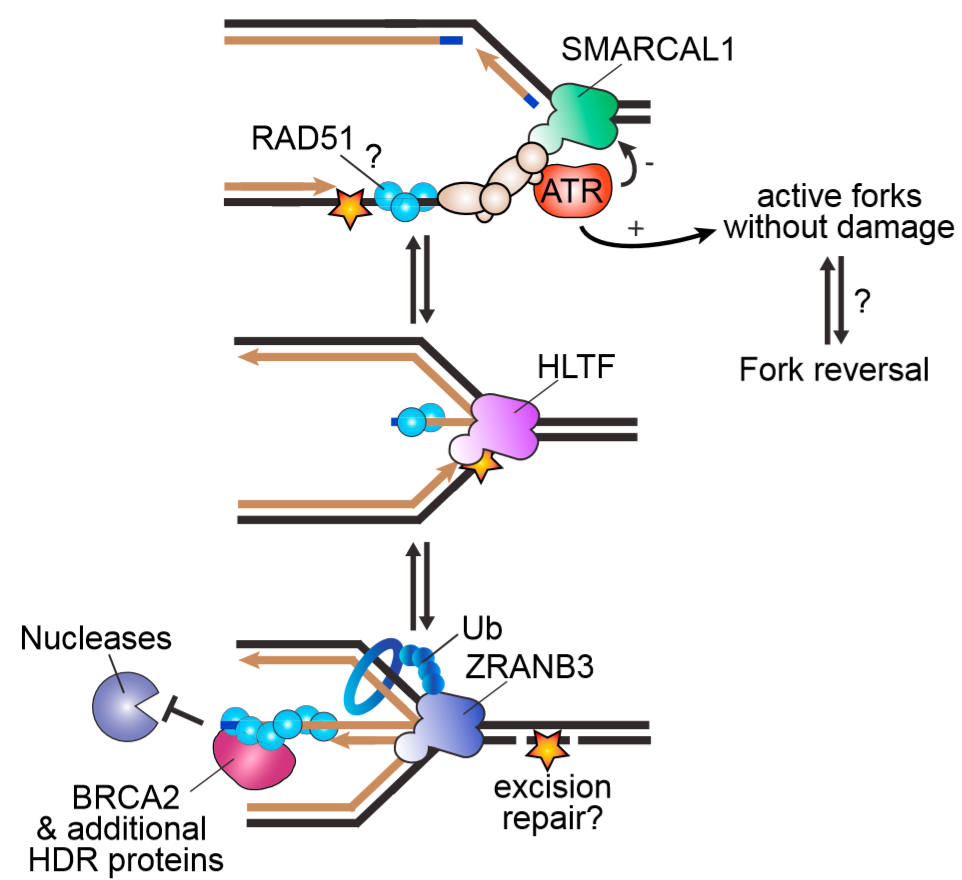
\includegraphics[width=0.56\textwidth]{resources/images/Intro/forkreversal.PNG}
    \caption[Schematic of Fork-reversal]{\textbf{Schematic of Fork-reversal.} Through fork reversal the damaged simplex DNA is placed back into a duplex context where the damage can be removed via excision repair. SMARCAL1, HTLF and ZRANB3 are regulated by RPA, 3' DAN ends and poly-ubiquitylated PCNA (see below) respectively. \citep{Cortez.2019}}
    \label{fig:forkreversal}
\end{wrapfigure}
Recombination proteins such as RAD51, BRCA1 and BRCA2 play crucial roles in fork-reversal pathways. \cite{Neelsen.2015} proposed that RAD51 binds ssDNA on the template strand start a coordinated annealing reaction (see Fig. \ref{fig:forkreversal}). \cite{Bhat.2018} on the other hand published some evidence on RAD51 capturing nascent ssDNA  as its formed by recombination proteins to shift the equilibrium towards fork-reversal.\\
Reversed forks aren't static constructs but can rather be processed by Double-Strand-Break repair nucleases like MRE11 or DNA2. Processing by those nucleases may remove end-binding proteins and therefore promote fork restart \citep{TeixeiraSilva.2017}. It has been shown that the MRE11-RAD50-NBS1 (MRN) nuclease binds to replication forks even in absence of exogenous DNA damage to interact with RPA but end-processing is mostly restricted by RAD51 to prevent nascent strand degradation \citep{Mijic.2017, Dungrawala.2015}. The actual actions of RAD51 at forks are heavily regulated by proteins including BRCA1, BRCA2 and the FANC proteins. The mentioned proteins promote RAD51-dependent fork protection but are not essential for fork-reversal. Negative regulation of RAD51 is done through RADX, FBH1 and BLM, indicating that repair mechanisms must not only be activated to act on specific lesion but they also need to be negatively regulated to prevent some effects of over-repair that can actually be more deleterious than the initial lesion \citep{Bhat.2018}.\\
The exact fate of the replication machinery during fork-reversal is not clearly known but there is some evidence for the dissiciation of the replisome \citep{Dungrawala.2015} whereas the CMG helicase most likely remains on the fork. This can be assumed due to the competence of most forks to resume replication quickly after prolonged blockage.\\\\
Fork reversal and lesion skipping may be independent mechanisms that could operate individually. How mammalian cells choose between the two pathways is not well studied yet. Post-translational modifications like ubiquitylation and sumoylation, especially to PCNA, are essential in pathway choice. ATR signalling also seems to play a critical role because reversal enzymes like SMARCAL1 are ATR substrates. Phosphorylation of SMARCAL1 by ATR for example has been shown to reduce its fork-remodelling activity \citep{Couch.2013}. \cite{Mutreja.2018} report an ATR-promoted stalling of forks that have not encountered any lesions by signalling from stalled forks.How exactly the reversal of undamaged forks benefits the cell even though it delays the completion of DNA replication is unknown.

\subsubsection{Resolution of Helicase-Blocking Lesions}
\label{sec:iclrepair}
Interstrand Crosslinks (ICLs) and DNA-Protein Crosslinks (DPCs), especially on the leading strand, pose a potent risk of fork blocking because they interfere with helicase unwinding, although they are much less common than polymerase-blocking lesions.\\
As already mentioned ICLs are formed in response to DNA-damaging agents that are used in cancer chemotherapy, such as Psoralen and mitimycin C, as well as through ionizing and UV radiation. Many effectors that can cause ICLs also cause DPCs. Additionally, interrupting the catalytic cycle of DNA-binding enzymes can lead to protein-DNA intermediates. Removal of those lesions by replication-coupled repair mechanisms is done through three main pathways.\\
One might expect complete blockage of replication fork movement in response to an ICL or DPC, but that is not the case. The CMG helicase encircles the leading strand and uses MCM10 as an accessory protein that helps to prevent lagging strand DPCs from blocking the helicase \citep{Langston.2017}. DPCs on the leading strand, that are be to big to physically be accommodated by the CMG channel, can also be traversed by the helicase via unwinding of DNA past the lesion by the accessory polymerase RTEL1 to provide a short ssDNA strand. This allows the MCM complex to bypass the DPC which promotes proteolysis-dependent repair of said lesion \citep{Sparks.2019}.\\
\begin{figure}[H]
    \centering
    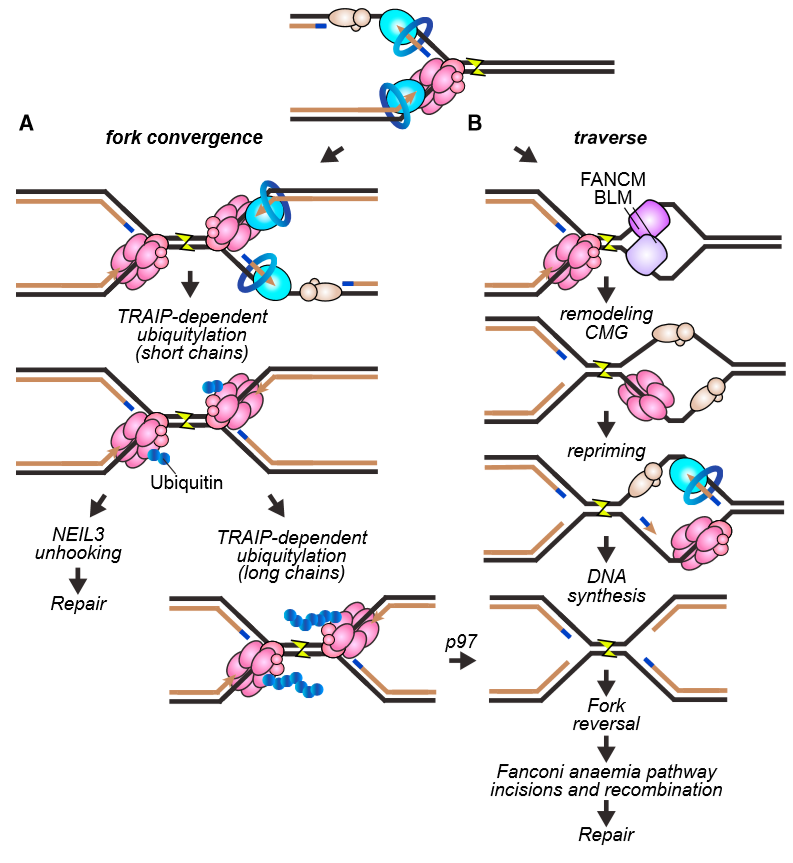
\includegraphics[width=0.7\textwidth]{resources/images/Intro/icl_replication.PNG}
    \caption[Replication-Coupled ICL Repair Mechanisms]{\textbf{Replication-Coupled ICL Repair Mechanisms.}\\
    A) Forks converge on an ICL, TRAIP-dependent short-chain ubiquitylation promotes recruitment of NEIL3 and leads to strand-unhooking. Long-chain ubiquitylation leads to unloading of the replisome followed by fork reversal and DNA incision via the Fanconi anemia pathway.\\
    B) ICL traversion via the use of FANCM and BLM as accessory helicases. Remodeled CMG helicase may allow traversal of the lesion followed by repriming of the MCM complex past the lesion. This leads the ICL to be repaired post-replicatively via the Fanconi anemia pathway.\\
    \citep{Cortez.2019}}
    \label{fig:iclrepl}
\end{figure}
ICLs also do not block the CMG helicase completely. The two additional helicases FANCM and BLM as well as the ATR kinase and FANCD2 can remodel the CMG helicase \citep{Huang.2013} in a way that allows "traversal" of interstrand corsslinks, although exact mechanisms for this have not been resolved yet \citep{Huang.2019}. The general mechanism of ICL traversal is similar to that of DPC traversal in that the CMG helicase may be blocked from unwinding DNA, but as long as another helicase provides ssDNA the MCM complex can reform past the lesion. Interestingly, ICL traversal can not be observed in \textit{Xenopus} egg extract systems which may be due to the high concentration of replication proteins that could disfavor ICL traversion.\\
DPC and ICl traversion lead generally to a similar situation to a base lesion which means that polymerases are stalled while the CMG helicase is able to continue unwinding DNA.Therefore repair of said ICL has to occur post-replicatively.  A DPC would not be lethal on its own wheras ICLs could interfere with chromosome segregation causing mitosis errors and cell death. Figure \ref{fig:iclrepl} shows possible replication-coupled mechanisms for ICL repair.\\\\
The two described possibilities for ICL handling during replication both end in X-shaped DNA structures around the crosslinks (see Fig. \ref{fig:iclrepl}). Unhooking of the crosslink is essential to complete replication and chromosome segregation and takes place through at least two independet pathways.\\
\begin{figure}[H]
\centering
    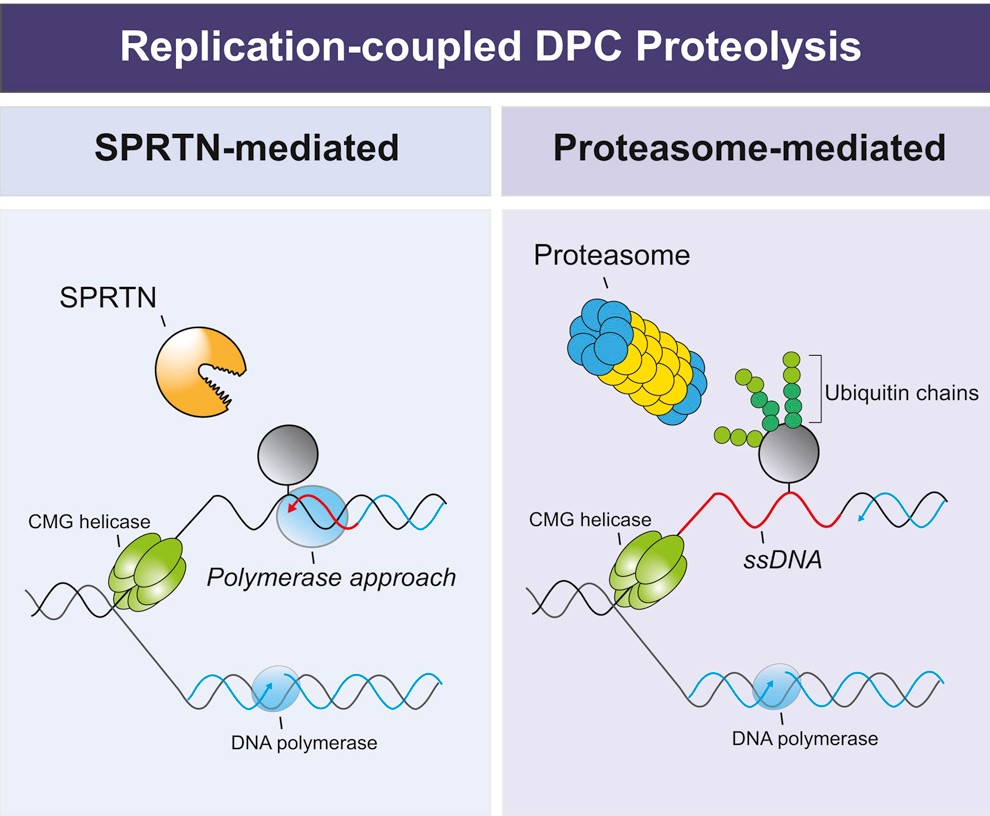
\includegraphics[width=.68\textwidth]{resources/images/Intro/sprtn.jpg}
    \caption[SPRTN- and Proteasome-mediated DPC Proteolysis]{\textbf{SPRTN- and Proteasome-mediated DPC Proteolysis.} SPRTN recognizes polymerase stalling on both the leading and the lagging strand and mediates DPC proteolysis similar to the yeast protease Wss1 \citep{Stingele.2015}. Proteasome-mediated proteolysis requires polyubuquitylation of the DPC.\\ \citep{Larsen.2019}}
    \label{fig:sprtn_action}
\end{figure}
Psoralen- and abasic site induced ICLs are mostly unhooked without DNA incision through NEIL3 \citep{Semlow.2016}. Unhooking via the NEIL3 glycosylase leaves an abasic site on one template strand and a mono-adduct or adenosine on the other. Those lesions are then repaired via TLS and some additional steps \citep{Raschle.2015}. Lesions introduces via other effectors are not good substrates for NEIL3 and have to be repaired via an alternative pathway involving a FANC protein-dependent mechanism. The FANC proteins get their name from the disorder that arises when one or more are inactivated called Fanconi anemia, that is characterized by cellular hypersensitivity to crosslinking agents \citep{Ceccaldi.2016}. This pathway requires the CMG helicase to be unloaded , the DNA backbone to be incised as well as the involvement of fork reversal \citep{Amunugama.2018}. Initially it was thought that BRCA1 was required for CMG helicase unloading but new evidence suggests that TRAIP catalyzes CMG ubiquitylation and therefore promotes p97-dependent unloading \cite{Wu.2019}.\\
DPC repair also requires further processing after lesion-traversion but because large DPCs block NER, at least two proteolysis-dependent mechanisms are required to resolve such lesions. Both of those mechanisms rely on SPRTN or the proteaseome \citep{Stingele.2016,Vaz.2016}.\\
Ubiquitylation of DPCs catalyzed by the E3 ligase TRAIP is neccessary to trigger proteasome activation. Sumoylation also regulates DPC repair but it is not well understood how nearby DNA-binding proteins are protected from proteasomal removal. Once proteasomal degradation is finished, the remaining small-peptide-crosslink can be excised by NER after the gap in the daughter strand is closed by a combination of Pol\textdelta~ and TLS polymerases. Because of this DPC repair via the proteasome is considered to be mutagenic.\\ An additional mechanism of DPC proteolysis has been described to be mediated by the metalloprotease SPRTN in eukaryotes \citep{Gao.2018}. SPRTN has been shown to act in a similar way to the yeast protease Wss1 \citep{Stingele.2015} meaning it recognizes polymerase stalling on both the leading and the lagging strand without the need for polyubiquitylation of the DPC the fork is stalling at \citep{Larsen.2019}.   
There is a possibility of topoisomerase proteins not completing their catalytic cicle which leads to them staying covalently bound to the DNA. Drugs like etoposide are considered topoisomerase poisons and greatly increase the frequency of such covalent bounds occuring. \cite{Pommier.2014} showed that those topoisomerase-DNA complexes are removed by tyrosyl-DNA phosphodiesterases (TDP1 or TDP2) that are regulated via ubiquitylation and sumoylation.

\subsubsection{Double Strand Break (DSB) Repair during replication}
Breaks in the DNA backbone are generated via multiple mechanisms during replication where any process that involves strand cutting can introduce DSBs. They can also be caused by structure-specific nucleases such as MUS81 that process persistently stalled forks \citep{Hanada.2007}.\\
In stark contrast to DSBs that form in cells in G\textsubscript{0} or G\textsubscript{1} phase, replication-associated breaks are mostly "single ended" in nature, meaning that recombination is the preferred mechanisms to resolve them. Breaks in the DNA strands caused during replication can be repaired using a process called Break Induced Replication (BIR) where a DNA resection followed by strand invasion can generate a fork structure that is capable of DNA synthesis using a modified replisome \see Figure \ref{fig:bir}.
\begin{figure}[H]
    \centering
    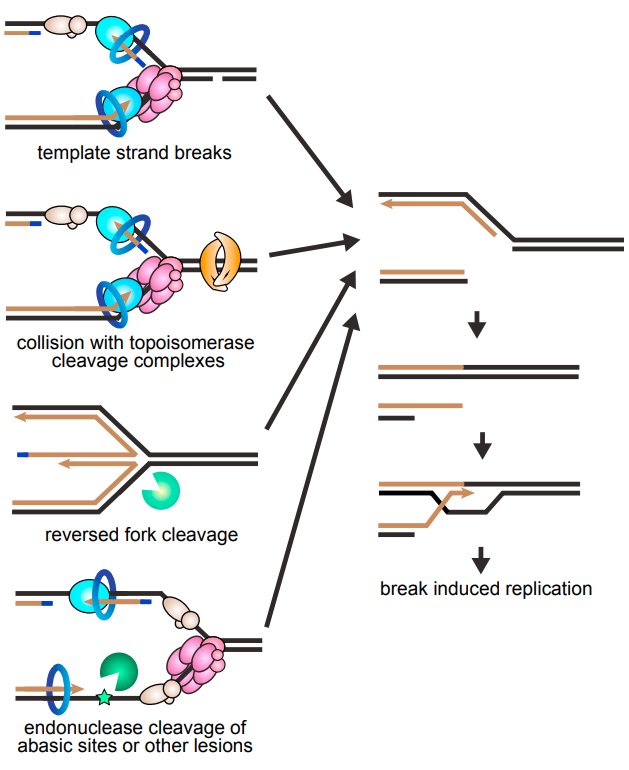
\includegraphics[width=.65\textwidth]{resources/images/Intro/bir.PNG}
    \caption[Mechanisms of DSB generation at Replication Forks]{\textbf{Mechanisms of DSB generation at Replication Forks. }Single-ended breaks are repaired by break-induced replication. The individual mechanisms depend heavily on an alternative replisome.\\\citep{Cortez.2019}}
    \label{fig:bir}
\end{figure}
BIR in general is best understood in yeast systems but has been studied in every eukaryotic organisms as well as in model system such as \textit{Xenopus} egg extracts. As a mechanisms involving strand invasion RAD51 plays a major role in BIR as well as an additional subunit of Pol\textdelta called POLD3 in humans or Pol32 in yeast. RAD51-dependent BIR mechanisms always involve RAD52 and are engaged at extraordinarily fragile sites. One example of this is when during replication MUS81 cleaves unreplicated DNA during mitosis. This underlines the idea that BIR is a mechanisms to prepare for mitosis and to facilitate chromosome segragation \citep{Bhowmick.2016}. Finally, BIR can be useful for telomere extension in cells using ALT where telomere damage induces a BIR replisome to replicate telomere sequences \citep{Dilley.2016}.

\subsubsection{Mismatch Repair}
Misincorporation errors are mainly repaired by mismatch repair (MMR). Base mismatches can by definition only occur on the daughter strand, therefore it is necessary to reliably distinguish the template from the daughter strand. In \textit{Escherichia coli} the template strand has a specific methylation pattern in the palindromic repeat sequence d[GATC] This enables excision and replacement of mismatched nucleotides  directed by the detection of a nick on the daughter strand caused by an error in this pattern \citep{Kunkel.2005}.\\
Similarly in eukaryotes, specifically in eukaryotic cell free extracts, mismatch repair is directed by a nick located 3' or 5' to the mismatch. The rate of mismatch repair is inverse proportional to the distance between the nick and the error from 125 to 1000 bp although repair was shown at much larger distances \citep{Iyer.2006}.\\
The actual repair of mismatched nucleotides is mediated by the redundant heterodimer MSH6-MSH3 that detects smaller insertion/deletion loops (IDLs) of 1-2 bp in cooporation with their obligate partner MSH2 whereas larger IDLs are detected by MSH2-MSH3. In addition to that MSH6-MSH3 interact with the DNA polymerase processivity factor proliferating cell nuclear antigen (PCNA) to localize MMR heterodimers to replication forks to repair replication errors as they occur. When MSH6-MSH3 encounters a DNA mismatch it undergoes a conformational change to a sliding clamp that diffuses along the DAN to free up mismatched nucleotides for recognition via MSH2-MSH6. This dimer recruits the heterodimer MLH1-PMS2 which in turn regulates the loading of the exonuclease Exonuclease 1 (Exo1) onto the daughter strand to promote excision of error-containing DNA fragments \citep{Gupta.2019}.
\newpage

\subsection{\textit{Xenopus} egg extracts as a Model System for Chromatin Proteomics}
\label{sec:extracts}
Studying proteins bound to chromatin is a crucial part of understanding the systemic and molecular mechanisms of DNA Repair and Replication. Even though systems like \textit{Xenopus} egg extracts have been used for decades to study different aspects of DNA processing using more traditional methods such as Western Blots and Immunostaining, the rise of mass spectrometry gave way to the field of high-throughput chromatin proteomics \citep{Blow.1990,Cupello.2016,Bonisch.2008}. One study that should be mentioned in the context of \textit{Xenopus} egg extracts in mass spectrometry is the large collaborative effort of M. Räschle, J. C. Walter, Z. Storchov\a'\ and M. Mann published in 2015 \citep{Raschle.2015} that explained how DNA crosslinks are detected and repaired using protein-chromatin interaction networks to resolve protein modules involved in crosslink repair.
\begin{figure}[H]
    \centering
    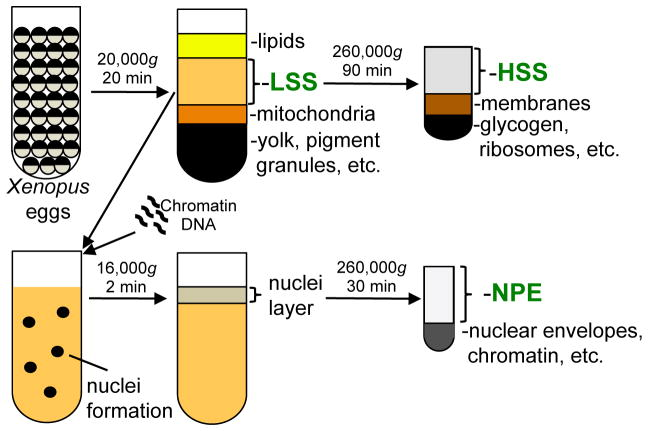
\includegraphics[width=.78\textwidth]{resources/images/Intro/extracts.jpg}
    \caption[\textit{Xenopus} egg extracts]{\textbf{\textit{Xenopus} egg extracts.} \textit{Xenopus} eggs are packed and then centrifuged at 20.000g for 20 min to separate lipids, mitochondria and yolk from the Low Speed Supernatant (LSS). Centrifugation of LSS at 260.000g for 90 min isolates the High Speed Supernatant (HSS) from the membranes and ribosomes. The addition of chromatin DNA to LSS leads to the formation of nuclei that can be separated from the rest of the mixture via a short centrifugation at 16.000g. An additional high speed centrifugation of the nuclei layer at 260.000g for 30 min separates the Nucleoplasmic Extract (NPE) from the nuclear envelops and the added chromatin.\\\citep{Cupello.2016}}
    \label{fig:extracts}
\end{figure}
\newpage
There are three main ways to prepare cell free extracts from \textit{Xenopus} eggs that are used to study specific aspects of chromatin processing. The easiest extract system to prepare is the so called Low Speed Supernatant (LSS) where eggs are packed and then centrifuged. This separates a yellow-brown mixture of protein, glycogen and membranes, the LSS extract, from the rest of the egg. Centrifuging LSS at high speeds separates the so called High Speed Supernatant (HSS) from membranes, glycogen and ribosomes. 
\begin{figure}[H]
    \centering
    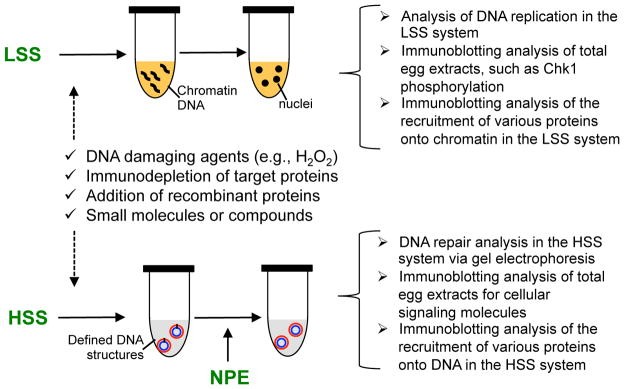
\includegraphics[width=.88\textwidth]{resources/images/Intro/extracts_uses.jpg}
    \caption[Usecases for \textit{Xenopus} egg extracts]{\textbf{Usecases for \textit{Xenopus} egg extracts.} Mixing LSS with chromatin DNA leads to the formation of nuclei that can be used to analyze DNA replication, for immunoblotting of total extracts and for proteomic analysis of protein recruitment to chromatin. Addition of substrate DNA to HSS forms the pre-replication complex (pre-RC) and licenses the added substrate for replication. After adding NPE DNA repair mechanisms can be analyse via gel electrophoresis while it is also possible to investigate protein recruitment and modification via proteomic methods.  \\\citep{Cupello.2016}}
    \label{fig:extract_uses}
\end{figure}
These extract systems deliver reliable tools to scientists studying the mechanisms of DNA repair and replication in a eukaryotic system that is closer to that of humans than fungal systems such as yeast, even though the molecular composition of the \textit{Xenopus} extract systems are not equal to unobstructed cells due to the treatments necessary for preparation. What extract system to choose for the experiment one wants to conduct depends heavily on these molecular differences and will be subject of later parts of this introduction (see Section \ref{sec:chromass} and \ref{sec:pp-ms}). As an example it should be mentioned that LSS as the simplest extract system is molecularly comparable to the embryonic interphase until sperm chromatin is added which initiates replication and therefore moves the extract to S-Phase (see Figure \ref{fig:cellCycle}.\\\\
In studies looking at the replication stress response of egg extracts LSS was treated with the endogenous regulatory protein Geminin which is synthesized during S phase to inhibit DNA replication by binding the initiation factor Cdt1 that cooperates with the ORC (origin recognition complex, \cite{Cook.2004}) to form the pre-RC complex (see section \ref{sec:cellcycle}.
\begin{figure}[H]
    \centering
    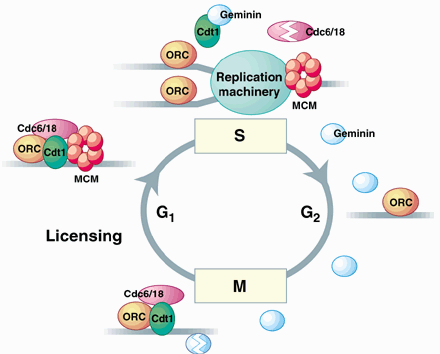
\includegraphics[width=.78\textwidth]{resources/images/Intro/gemininCell.png}
    \caption[Schematic depiction of a cell cycle showing the action of Geminin.]{\textbf{Schematic depiction of a cell cycle showing the action of Geminin. } During S phase once DNA replication started the regulatory protein Geminin is expressed. Geminin binds to Cdt1 and therefore inhibits the formation of the pre-RC to prevent the replication of already replicating DNA molecules. Geminin expression is kept up throughout G\textsubscript{2} but is decreased in M to allow effective chromatin licensing in G\textsubscript{1}. \citep{Lygerou.2000}}
    \label{fig:geminin}
\end{figure}
Even though HSS and NPE are essentially different extracts, they have to be mixed to study replication-dependent mechanisms due to the fact that HSS mostly contains proteins neccessary to form the pre-RC complex and NPE does not. Without the addition of HSS to NPE DNA replication can not start because no origin licensing can occur (\cite{Lebofsky.2009} and Figure \ref{fig:replication_overview}). 
Therefore they can be considered as one system --- referenced henceforth as the NPE/HSS system --- even though non-replicating extracts are rising in popularity due to the possibility to study replication-independent repair mechanisms as well as interaction of different ATPases with DNA (unpublished studies, J.C. Walter \& M. Räschle).

\subsubsection{CHROmatin MASS Spectrometry}
\label{sec:chromass}
The CHROMASS (Chromatin Mass Spectrometry) system established by \cite{Raschle.2015} uses \textit{Xenopus} egg extracts described in \ref{sec:extracts} to analyse chromatin bound proteins using mass spectrometry. CHROMASS can therefore be used to analyse the time-dependent recruitment of proteins to chromatin under different conditions to characterize repair- and replication mechanisms.
\begin{figure}[H]
    \centering
    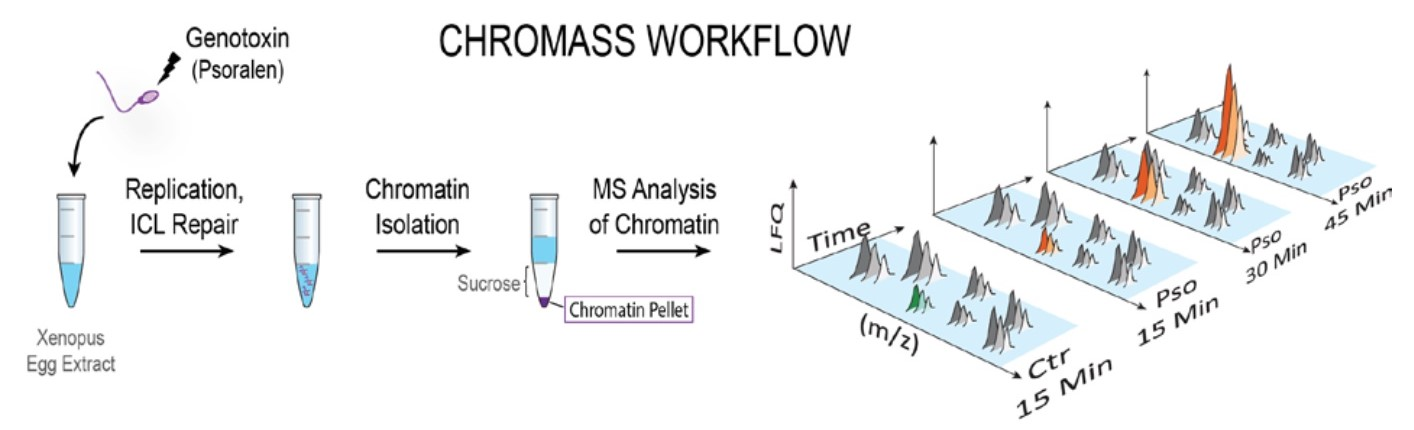
\includegraphics[width=0.98\textwidth]{resources/images/Intro/chromass.PNG}
    \caption[CHROMASS workflow.]{\textbf{CHROMASS workflow.} Genotoxin-treated sperm chromatin is added to \textit{Xenopus} egg extracts to initiate replication and repair. Chromatin is isolated after incubation for 15, 30 and 45 min via centrifugation through a sucrose cushion. The proteins bound to chromatin are isolated, digested, desalted and measured via mass spectrometry.\\ \citep{Raschle.2015}}
    \label{fig:chromass}
\end{figure}
Figure \ref{fig:chromass} shows the workflow used by \cite{Raschle.2015} to characterize the dynamic complex assembly during ICL bypass. Generally, damaged or undamaged sperm chromatin is added to \textit{Xenopus} egg extracts and then kept at room temperature (RT) to initiate replication and repair of added DNA. The chromatin is then separated from the mixture after set time points after initial addition by centrifuging through a sucrose cushion. Chromatin-bound proteins are then purified and a tryptic digest followed by a desalting step are performed. The purified peptides are then measured via mass spectrometry. For this kind of study, all of the three extract systems described in section \ref{sec:extracts} can be used to study protein recruitment in a time-dependent manner. MS DATA LOOKS LIKE TRADITIONAL RESULTS --> CHROMASS WORKS!

\subsubsection{Plasmid-Pulldown Mass Spectrometry}
\label{sec:pp-ms}
\begin{wrapfigure}{r}{.5\textwidth}
    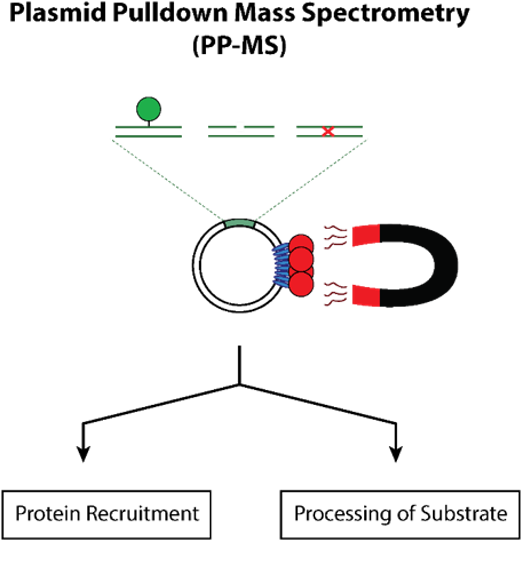
\includegraphics[width=.48\textwidth]{resources/images/Intro/pp-ms.png}
    \caption[Plasmid-Pulldown Mass Spectrometry workflow]{\textbf{Plasmid-Pulldown Mass Spectrometry workflow.}The plasmid substrate contains defined lesions and multiple repeats of a \textit{lacI}-binding sequence. After incubating the reaction mixture for the desired time a defined volume is removed and combined with beads coupled to \textit{lacI} which binds the plasmid substrate and therefore all DNA-bound proteins. The beads are then processed for mass spectrometry or loaded onto gels to visualize substrate processing (modified, Markus Räschle).}
    \label{fig:pp-ms}
\end{wrapfigure}
Plasmid-Pulldown Mass Spectrometry (PP-MS) is a system closely related to CHROMASS, although it has been shown that only the NPE/HSS system reliably replicates the plasmid DNA used for this method. Generally, plasmids with defined lesions are added to NPE/HSS and incubated to allow replication and repair. Isolation of this template DNA is achieved via a pull-down system which is enabled by the inclusion of a \textit{lacI}-binding site on the plasmid. The reaction mixture is added to \textit{lacI}-coated beads that bind to the \textit{lac}-operon fragment on the plasmid. The mixture is washed multiple times to remove unbound molecules after which the beads were dried and prepared for mass spectrometry in a similar fashion to the methods described in section \ref{sec:chromass}.\\
In addition to the proteomic analysis PP-MS can also be used to process the substrate DNA via gel electrophoresis to visualize replication kinetics (Fig. \ref{fig:pp-ms}).\\ 
This system has recently been used to describe the mechanism of SPRTN- and Proteasome-mediated replication-dependent DNA-Protein crosslink repair in \textit{Xenopus} egg extracts \citep{Larsen.2019}. The main benefit of PP-MS over CHROMASS is the ability to create specific lesions on the substrate in comparison to mostly unspecific lesion on sperm chromatin treated with genotoxins. Additionally, the repair of the lesion takes place over a shorter time-frame because plasmid DNA has a significantly faster replication kinetic due to its structure and size and its independence of prior chromatin assembly in \textit{Xenopus} egg extracts \citep{Sanchez.1992, AquilesSanchez.1995}. Using protein binding motifs on the plasmid templates it is also possible to synchronize their replication.\\

\subsection{Big Data and Networks in Biological Research}
Methods such as the ones described in the sections above create large amounts of data that have to be processed and handled correctly. Big Data, as the aggregate of such large datasets tends to be called, is used to draw conclusions from individual collections of data as well as the entirety of those collections.\\
Advanced computational methods such as the ones used by NCI in the development of TCGA can help understand biological systems using data gathered by 'omics experiments such as CHROMASS or PP-MS. Identification of key regulatory factors and mechanisms is crucial in resolving those systems and can be directly achieved by for example co-expression analysis in the case of gene expression data. Co-expression analysis algorithms can also be applied to  CHROMASS and PP-MS data sets under the assumption that proteins found on chromatin are recruited to it under specific conditions. This enables one to identify functionally similar proteins due to their similar chromatin binding pattern. The similarity of data collected for different proteins in one or more experiments can then be visualized in form of a protein-protein or gene co-expression network.
\subsubsection{Network visualization using correlation algorithms}
The following section is based on \cite{Dytham.2011} unless specified otherwise.\\\\
A relatively simple way to tackle co-expression analysis is correlation which is a measure of the relationship between two variables. Pearson's r correlation is the most widely used correlation statistic to measure the degree of relationship between variables that are linearly related. Pearsons correlation coefficient $r$ is calculated using the following equation.\\
\begin{equation}
    r_{xy} = \frac{n\sum x_i y_i - \sum x_i \sum y_i}{(\sqrt{n\sum x_i^2-(\sum x_i)^2}\sqrt{n\sum y_i^2-(\sum y_i)^2}}
\end{equation}
$r_{xy}:$ Pearson r correlation coefficient between $x$ and $y$\\
$n:\text{number of observations}$\\
$x_i:\text{value of $x$ (for ith observation)}$\\
$y_i:\text{value of $y$ (for ith observation)}$\\
\\
Pearson correlation only works based on the assumption that both variables are normally distributed and have a linear relationship. Additionally, the data has to be homoscedastic meaning it has to be equally distributed along the regression line. Given these assumptions Pearsons $r$ can be useful to investigate biological mechanisms up to more complex relationships such as protein-chromatin interaction networks.\\
The calculated correlation matrix for a set of variables can then be visualized in form of a network where the nodes represent variables and the edges their relationship. Additionally it is possible to use grouping algorithms such as Hierarchical Clustering to look at especially highly correlating variables.\\
To minimize computational effort and to reduce noise in the data set it is necessary to filter the gathered correlation matrix by the coefficient as well as the p-value. Determining the thresholds for filtering is another challenge in itself that can be tackled in different ways.\\
The simplest and most dangerous method of filtering networks for ease of visualization is setting a fixed correlation threshold. This is known as \textit{hard thresholds} where all edges of the network are filtered in such a way that all edges with $x \geq \tau$ are included. This method produces simple results that come with the danger of losing meaningful information depending on the threshold. If one sets $\tau = 0.7$ it is possible to lose a meaningful edge that has a weight of $0.6985$ \citep{Carter.2004}.\\
Another option is filtering for statistical significance of the calculated correlation coefficient based on the assumption that they are normally distributed meaning that the probability density function follows:\\
\begin{equation}
    f(x)=\frac{1}{\sigma \sqrt{2\pi}}e^{-(x-\mu)^2/2\sigma^2}
\end{equation}
$\sigma:\text{standard deviation}$\\
$\mu:\text{mean}$\\
\\
The p-value itself describes the probability of obtaining test results that are at least as extreme as the actually achieved results, meaning that it tells one if an observation could have also been done at random. An observation can be seen as statistically significant if $p < 0.05$ and highly significant if $p < 0.01$, stating that the probability making said observation at random is below 5\% or 1\% respectively.
For Pearson's $r$ this can be done relatively easily because the p-value for this measure of correlation uses the t-distribution. In this case $H_0:p=0$ vs. $H_1: p\ne0$ where $p$ is the correlation value between two variables.\\
\begin{equation}
    t = \frac{r\sqrt{n-2}}{\sqrt{1-r^2}}
\end{equation}
$r:\text{correlation coefficient}$\\
$n:\text{number of observations}$\\
\\
Where the p-value is $2*P(T>t)$ with T following a t-distribution with $n-2$ degrees of freedom.\\
The correlation matrix can then be filtered to include all relationships where $p(x) \geq \rho$ with an established p-value threshold in biological relationships of $0.01$.\\
After filtering the correlation matrix is transformed to an adjacency matrix using a sigmoid function where the correlation or rank interval $[-1,1]$ is mapped to $[0,1]$.\\
\begin{equation}
    a_{xy}=signum(s_i, \tau) \equiv 
    \begin{cases}
        1 & \text{if $s_{xy} \geq \tau$}\\
        0 & \text{if  $s_{xy} < \tau$}
    \end{cases}
\end{equation}
The two filtering methods work reliably in combination with one another if optimized correctly but can, as already mentioned, lose meaningful information. One way to prevent this is to implement soft thresholds such as the sigmoid function used here.\\
\begin{equation}
    a_{xy}=sigmoid(s_i,\alpha,\tau_0)\equiv\frac{1}{1+e^{-\alpha(s_{xy}-\tau_0}}
\end{equation}

\subsubsection{Weighted Correlation Network Analysis}
Weighted Correlation Network Analysis also known as weighted gene co-expression network analysis (WGCNA) is an established method for the identification of modules and intermodular hubs mostly used in genomic applications \citep{Horvath.2011}.\\
It was developed by Steve Hovarth and his colleagues at the UCLA Fielding School of Public Health as a means to expand on the previously unweighted methods of network analysis. The benefits of using weighted correlation network analysis over an unweighted analysis start with the use of a sigmoid adjacency function to apply a soft threshold that is data dependent to prevent data loss. Additionally, a topoligocal overlap measure is calculated from a the adjacency matrix that has been shown to more precisely represent gene co-expression. The construction of networks using this method delivers highly robust results if the parameters of the soft threshold are changed meaning that an optimization of the sigmoid adjacency function is not necessary for brief data analysis \citep{Zhang.2005}. It can also be used to enhance standard data-mining methods such as cluster-search since similarity measures can often be transformed to weighted networks \citep{Oldham.2012}.\\\\
Most recently, WGCNA in conjunction with an optimized adjacency function was used to visualize a co-regulation map of the human proteome with which they could identify the function of novel proteins \citep{Kustatscher.2019}. To achieve this goal they combined WGCNA with a tree-based clustering algorithm published by \cite{Buttrey.2015} that improves co-regulation analysis by using the Jaccard similarity coefficient as a measure of similarity \citep{Gupta.2018}. The Jaccard coefficient is defined as:\\
\begin{equation}
    J(A,B) = \frac{|A \bigcap B|}{|A \bigcup B|}
\end{equation}\\
From this coefficient the so called Jaccard metric can be deduced.\\
\begin{equation}
    J_\delta(A,B) = 1 - J(A,B) = \frac{|A \bigcup B|-|A \bigcap B|}{|A \bigcup B}
\end{equation}\\
By applying this combination of methods to a large collection of SILAC experiments they were able to provide an interactive resource for scientist to browse the human protein interactome and to deduce the functions of not well studied proteins by their association using the principle of "Guilt-by-association" described in Figure \ref{fig:co-expression}.\\\\
In this study we assumed that the methods applied by \cite{Kustatscher.2019} can be used to analyze the regulation of chromatin binding under specific DNA damage conditions to identify novel repair factors or to give mathematical support to experimentally found associations. 

\subsubsection{Predicting Protein Functions using Networks}
\textit{The following section is based on \cite{Gillis.2012} unless stated otherwise.}\\\\
It is mostly thought that gene functions have to be studied in the context of networks. Networks consisting of millions of interactions gathered from RNA coexpression analysis, protein binding assays and other high-throughput methods can be studied using freely available data only have been embedded in a large number of studies published by molecular biologists all over the world. Most of these studies combine these networks with codifications of gene function (i.e. Gene Ontology). If the information derived from the network overlaps with the annotation of a gene one might assume that the genes must have a similar function but to understand the actual function of a gene in the whole systemic context one has to look at all interactions of a gene or protein.\\
Biologists have dealt with this problem by leveraging the "Guilt-by-association" principle (GBA). GBA states , as mentioned in Figure \ref{fig:co-expression}, that it is possible to use a network representation of complex protein relationships to deduce the function of an unknown protein from the ones it correlates with. This can in theory be applied to biological data of any "level", meaning it can be used to analyze genomic, transcriptomic, proteomic and metabolomic data \citep{Oliver.2000}.\\ The performance of GBA in a purely computational applications is commonly assessed using cross-validation where known functions are masked from part of the network followed by measuring the ability to recover the masked information. This is known as the concept of "Precision-recall". The area under a Precision-recall curve is useful to evaluate the performance of identification algorithms because it is very sensitive to the effects of a single highly-ranked correct guess. This means that precision-recall rewards methods that provide one good prediction while subsequent errors have much less effect on the evaluation \citep[S1]{Gillis.2012}. In our case we used the "average precision" (AP) as a metric for GBA performance based on the findings of \cite{Gillis.2012}. It is calculated using:\\
\begin{equation}
    AP = \frac{1}{k}\sum_{i=1}^{k} \frac{i}{rank_i}
\end{equation}\\
Another option of estimating the performance of grouping algorithms in graph theory is to simply compare computational results with known experimental results. A strong similarity between experimental and computational data given integrity of both data sources suggests a good performance of an algorithm for that specific type of data. For this to be considered a reasonable approach one has to first verify the integrity of the underlying data and check if the sets themselves are comparable. \\
There are multiple algorithms for the identification of protein modules, two of which will be explained and used in this thesis.

\subsection{Clustering algorithms for the identification of functional protein modules}
\label{sec:diffusion}
Generally the assumption one has to make before using clustering algorithms on biological networks of any kind is that items in the network that are close to each other are thought to behave similarly. This \textit{closeness} can either be a direct neighborhood or a connection over a low number of nodes between two items. To group individual items of a network together, one has a multitude of options depending on their use case. In the field of chromatin proteomics a network item describes a protein while each edge between two items or nodes describes a measure or co-binding or co-regulation. The simplest method of clustering nodes in biological networks is an algorithm called "Nearest Neighbor Clustering". Functionally, it selects all nodes that are directly connected with an input node. While effective, this algorithm has a high false discovery rate due to its reliance on the correct preparation of the network it is used on. When a network contains a lot of edges that are biologically speaking insignificant, the probability of a number of resulting nodes in the cluster being there by chance is high. On the other hand, proteins that are important for the function of another protein but are connected through longer paths to the starting node, they are not included.\\
An improvement over Nearest Neighbor Clustering are "Shortest Path" algorithms like Bellman Ford that are used to determine the distance of nodes to an input node - henceforth called "query". The resulting path lengths are then ranked to reduce the false positive rate and improve the ability to draw meaningful conclusions from the clustering result \citep{Franke.2006}.
\begin{figure}[H]
    \centering
    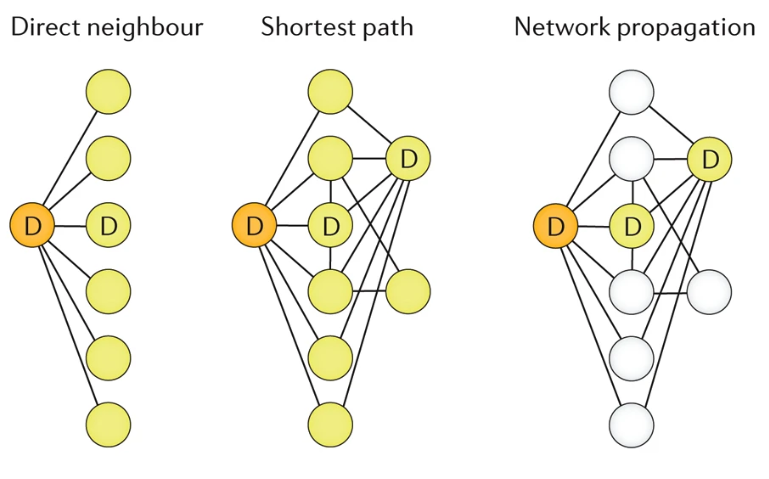
\includegraphics[width=.6\textwidth]{resources/images/Intro/clustering_methods.PNG}
    \caption[Schematic example of neighborhood clustering, shortest path search and network propagation]{\textbf{Schematic example of neighborhood clustering, shortest path search and network propagation. }A single network node (D, orange) with a known function is used to identify other potential functionally related nodes (D, yellow).\\\citep{Cowen.2017}}
    \label{fig:clustering_methods}
\end{figure}
While the two methods described above can yield presentable results for simpler applications they should only be used to quickly analyze more complex data. Predicting relationships and functional interactions in complex biological networks by means of simple mathematical clustering be it scored or not is not feasible due to the high amount of processing that has to be done to the data to decrease the amount of false positives and negatives. \cite{Cowen.2017} showed that \textit{Network Propagation} is a better way to mine data using complex biological networks. Functionally, Network Propagation transforms a list of query proteins into a proteome-wide profile of similarly regulated proteins. In our case this method can be applied to find proteins that have a similar chromatin binding pattern under specific damage conditions. 
\begin{figure}[H]
    \centering
    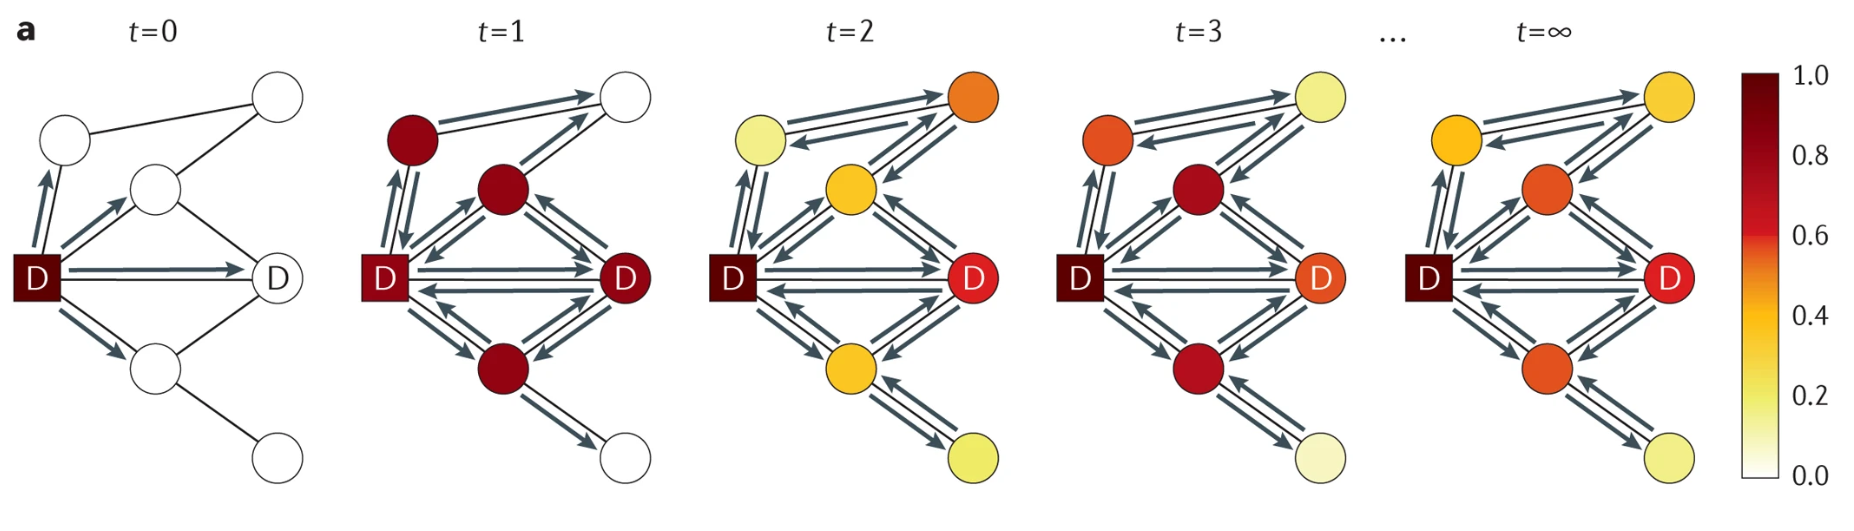
\includegraphics[width=\textwidth]{resources/images/Intro/network_propagation.PNG}
    \caption[Step-by-step demonstration of network propagation]{\textbf{Step-by-step demonstration of network propagation. } Propagation process is shwon at different time points until a steady state is reached ($t=\infty$) and arrows depict the direction of the walk flow. Nodes are colored according to the amount of flow they recieve. D indicates nodes with a known function (square) or with predicted functions (circle).\\\citep{Cowen.2017}}
    \label{fig:network_propagation}
\end{figure}
Network propagation uses a list of proteins with a known function as a query. The have been shown to be capable of identifying previously unknown or predicted disease-associated genes in complex networks ranging from cancer patient data to Alzheimer's research collections \citep{Cowen.2017}. One algorithm belonging to this class is the Google PageRank algorithm \citep{TaherHaveliwala.2003}.
The algorithm gives the query nodes a score of $1.0$ and the score of all other nodes to $0.0$. It then walks along the edges of the network starting at one of the query nodes and at every step each node diffuses its score to its neighboring nodes where the amount it diffuses is proportional to the weight of the edge in weighted networks. This algorithm has been implemented by \cite{Menges.2018} and will be used to mine the DNA Repair Atlas for functional DNA repair modules.
\subsection{Dimensionality Reduction and its applications in High-Throughput Data Analysis}
In addition to analyzing the co-regulation or co-expression of proteins it is often wise to analyze the relationship of the individual experiments that are part of a meta-analysis. For example, a collection of 48 proteomic experiments consisting of about 400 measurements in total with around 5000 proteins identified per measurement can be represented as a matrix with 96,000,000 dimensions. The relationship between the different conditions can teach a data scientist about the integrity of each set and allows , for example, filtering for outliers. In general, dimensionality reduction is used to identify driving components of high-dimensional data sets (i.e. Principle Component Analysis) or to visualize the relationship of individual sets in large collections (i.e. t-Distributed Stochastic Neighbor Embedding) as demonstrated by \cite{Kustatscher.2019}.

\subsubsection{t-Distributed Stochastic Neighbor Embedding}
t-Distributed Stochastic Neighbor Embedding (t-SNE) is a non-linear dimensionality reduction algorithm that has been implemented in different programming languages to be used in multiple data analysis toolkits. It was initially developed as a machine learning algorithm for visualization by L. van der Maaten and G. Hinton \citep{vanderMaaten.2008} that is especially useful for visualising relationships between high-dimensional datasets in a low-dimensional space. t-SNE is comprised of two main steps:\\
A probability distribution over pairs of high-dimensional objects is constructed in such a way that similar objects have a high probability of being selected.\\
After that similar distributions are constructed for a low-dimensional map and the one with the lowest "Kullback-Leibler divergence" with respect to the position of map points to the high-dimensional map is selected. Due to simplicity, the mathematical details of the algorithm are not shown here but can be found in the paper linked above.\\
t-SNE is a useful tool for working with large collections of data because it allows the comparison of individual parts of the collection with one another on a low-dimensional map. This is especially the case if one wants to identify local structures of complex collections i.e. the relationship between different replicates or treatment conditions in one of the included experiment sets while still maintaining information about the global structure of the data collection \cite{Kobak.2019}. In this thesis this algorithm was used to see whether the experiment sets included in the atlas can be compared with one another without loosing information about the individual sets themselves.